\begin{figure}[h]
  \begin{center}
    \begin{tabular}{ccc}
      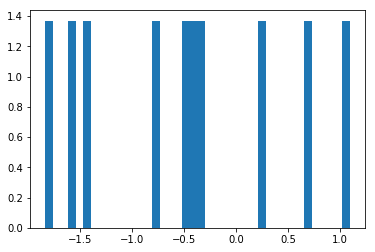
\includegraphics[width=0.32\hsize]{figure/10_1.png} &
      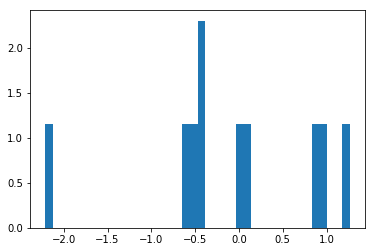
\includegraphics[width=0.32\hsize]{figure/10_2.png} &
      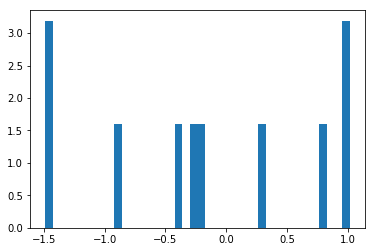
\includegraphics[width=0.32\hsize]{figure/10_3.png} \\
      試行1 & 試行2 &試行3
    \end{tabular}
    \caption{標準正規分布に基づく10個の乱数のヒストグラム}
    \label{figure1}
  \end{center}
\end{figure}
\begin{figure}[h]
  \begin{center}
    \begin{tabular}{ccc}
      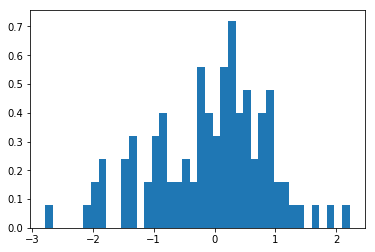
\includegraphics[width=0.32\hsize]{figure/100_1.png} &
      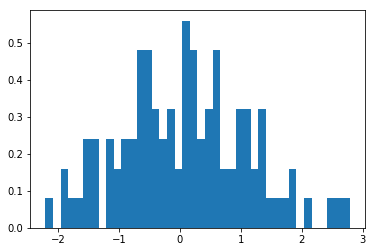
\includegraphics[width=0.32\hsize]{figure/100_2.png} &
      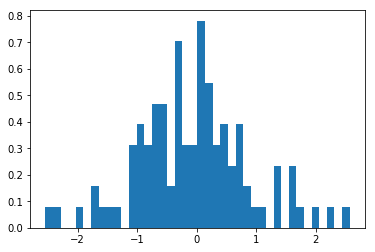
\includegraphics[width=0.32\hsize]{figure/100_3.png} \\
      試行1 & 試行2 &試行3
    \end{tabular}
    \caption{標準正規分布に基づく100個の乱数のヒストグラム}
    \label{figure1}
  \end{center}
\end{figure}
\begin{figure}[h]
  \begin{center}
    \begin{tabular}{ccc}
      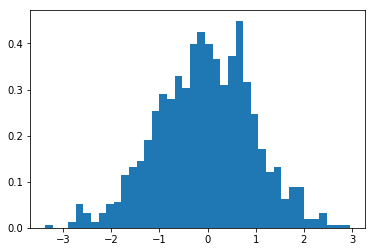
\includegraphics[width=0.32\hsize]{figure/1000_1.png} &
      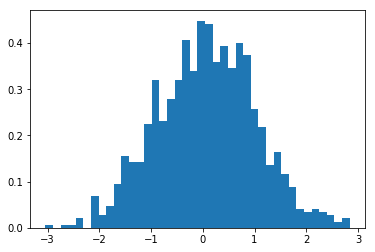
\includegraphics[width=0.32\hsize]{figure/1000_2.png} &
      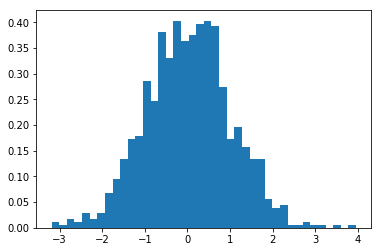
\includegraphics[width=0.32\hsize]{figure/1000_3.png} \\
      試行1 & 試行2 &試行3
    \end{tabular}
    \caption{標準正規分布に基づく1000個の乱数のヒストグラム}
    \label{figure1}
  \end{center}
\end{figure}
\begin{figure}[h]
  \begin{center}
    \begin{tabular}{ccc}
      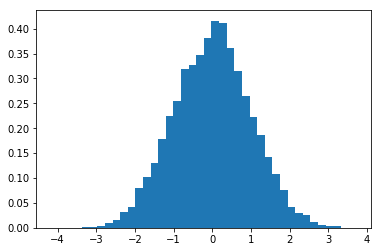
\includegraphics[width=0.32\hsize]{figure/10000_1.png} &
      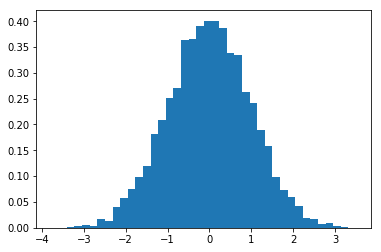
\includegraphics[width=0.32\hsize]{figure/10000_2.png} &
      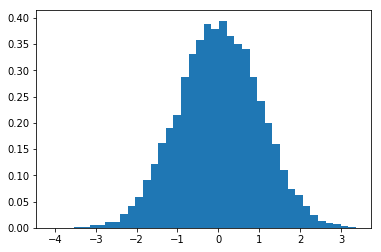
\includegraphics[width=0.32\hsize]{figure/10000_3.png} \\
      試行1 & 試行2 &試行3
    \end{tabular}
    \caption{標準正規分布に基づく10000個の乱数のヒストグラム}
    \label{figure1}
  \end{center}
\end{figure}
